% !TEX root = ../main.tex

\section{Use case diagram}
\label{sec:usecase}

Er zijn twee use cases een voor de desktop / mobile app en een voor de server. 
Bij de desktop / mobile app zijn er 4 actoren. Als eerste de admin die accounts 
moet kunnen beheren en authentiseren en synchroniseren met de server. 
Dan is er de user die alle bestanden, agenda’s, media en rechten moet kunnen 
beheren en ook moet authentiseren en synchroniseren met de server. Er is ook 
een media speler die media moet kunnen opvragen. En als laatste is er ook de 
server die moet kunnen synchroniseren met de admins en users.
Er is ook een use case voor de server. Bij de server zijn er 3 actors de eerste 
is de client die bestanden, media, agenda’s, accounts en rechten moet kunnen 
opvragen en beheren. De client moet zich ook kunnen authentiseren. Dan is er 
ook de version control die bestanden moet kunnen opvragen en beheren en zich 
ook moet kunnen authentiseren. Uiteindelijk is er ook de admin die accounts en 
rechten moet kunnen opvragen en beheren en zich moet authentiseren.

\begin{figure}[H]
  \centering
  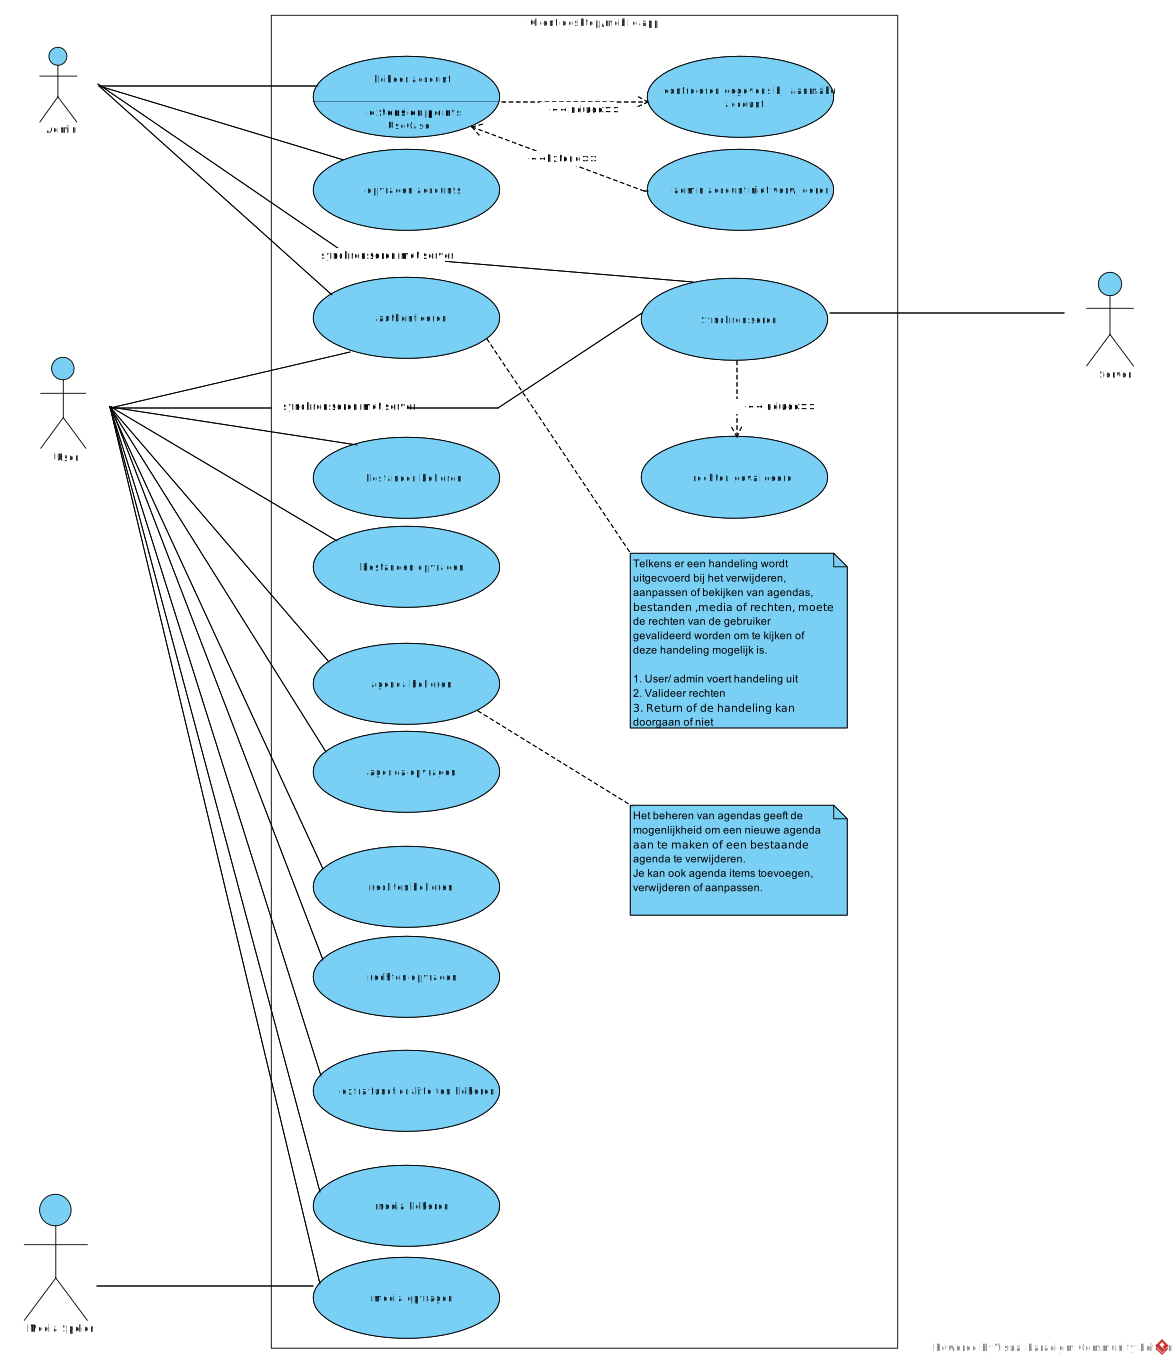
\includegraphics[width=1\textwidth]{images/usecase1.png}
  \label{figure:usecase1diagram}
\end{figure}

\begin{figure}[H]
  \centering
  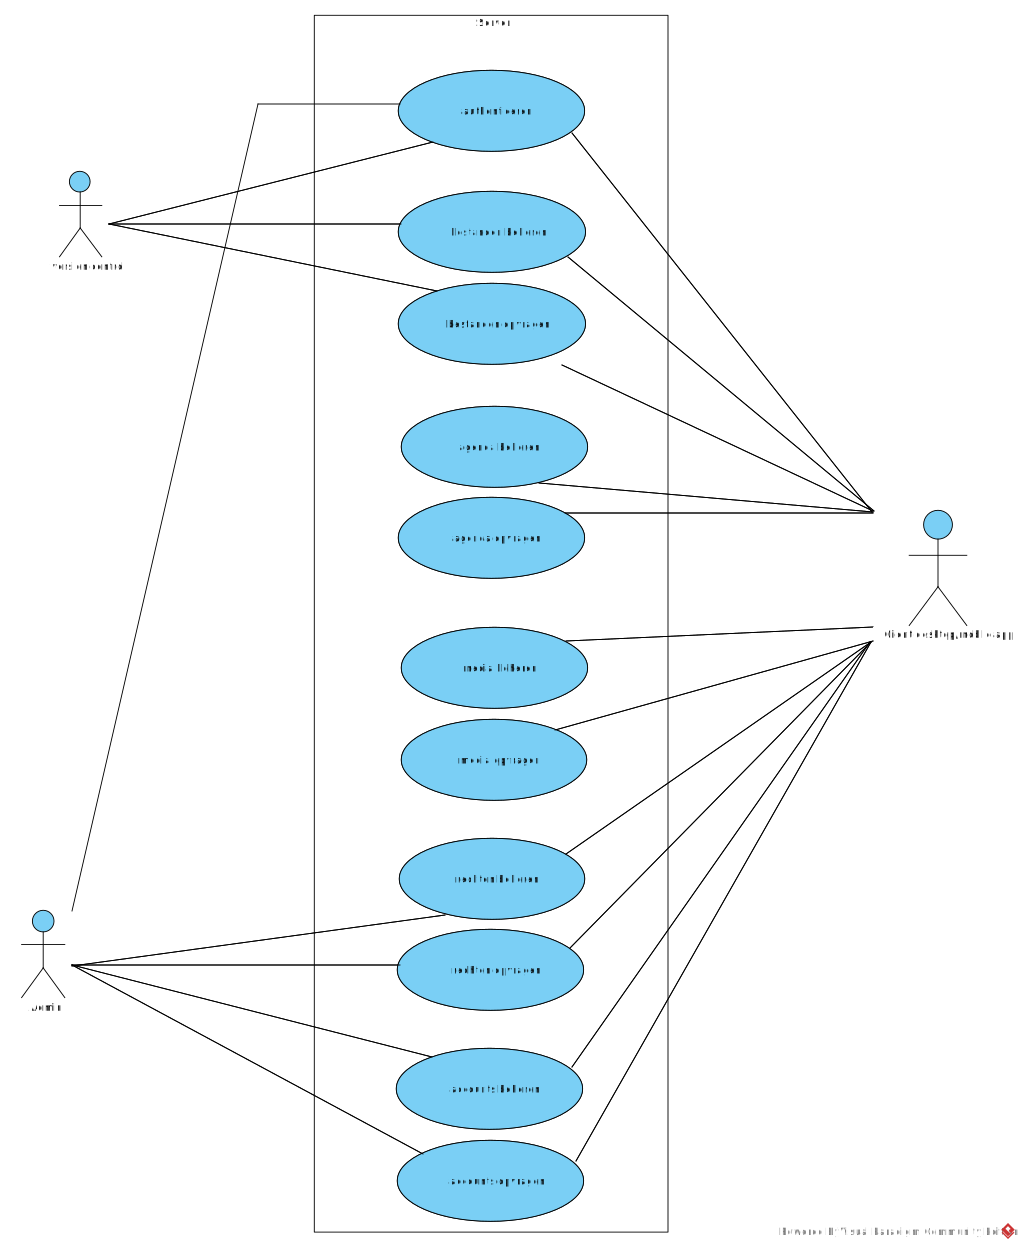
\includegraphics[width=1\textwidth]{images/usecase2.png}
  \label{figure:usecase2diagram}
\end{figure}

\newpage

\section{Domein class diagram}
\label{sec:domeinclass}

In het klasse diagram worden enkele klassen van de desktop / mobile app 
beschreven. Je hebt de persoon klasse waar de user en admin klasse van afgeleid 
zijn. De persoon klasse communiceert met de server waar een authenticator 
klasse de rechten valideert. De user klasse heeft agenda’s, een media 
bibliotheek en een bestands bibliotheek voor lokale gegevens. De users kan hier 
gegevens downloaden en uploaden via de server connectie. En de media 
bibliotheek heeft ook een associatie met een externe media speler om de media 
weer te geven.

\begin{figure}[H]
  \centering
  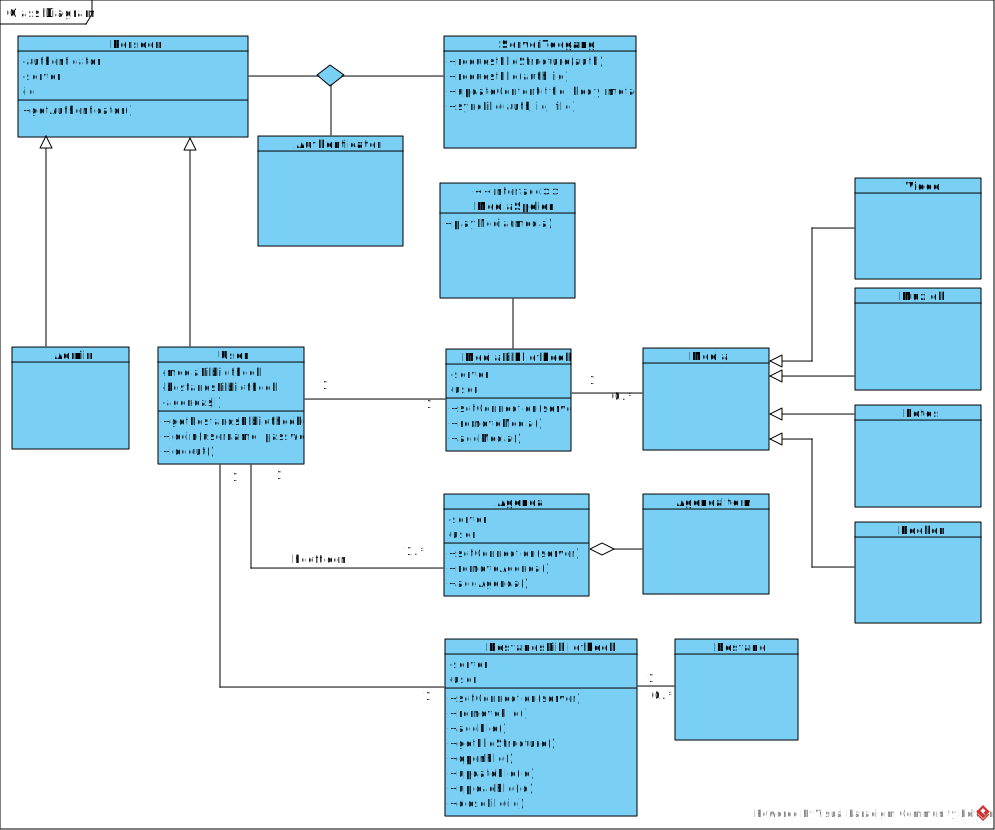
\includegraphics[width=1\textwidth]{images/classdiagram.png}
  \label{figure:classdiagram}
\end{figure}

\newpage

\section{Sequentiediagram}
\label{sec:sequentie}

Het sequentiediagram geeft weer hoe een niet lokaal bestand aangepast kan worden.
Hierbij wordt een authenticator opgezet die de connectie met de server kan valideren.
Omdat het bestand niet lokaal bestaat zal de mediabibliotheek het bestand ophalen, editeerbaar maken en terug uploaden.

\begin{figure}[H]
  \centering
  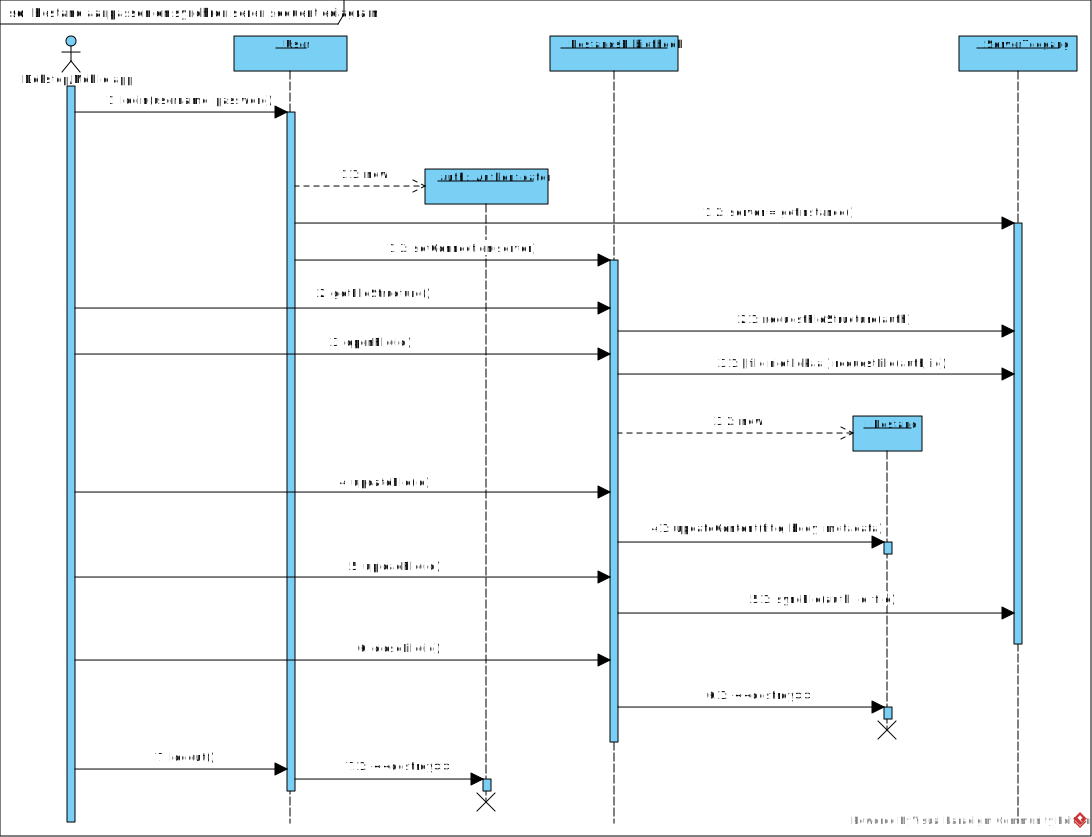
\includegraphics[width=1\textwidth]{images/sequentiediagram.png}
  \label{figure:sequentiediagram}
\end{figure}

\newpage

\section{Activiteitendiagram}
\label{sec:activiteiten}

Het activiteitendiagram toont aan hoe een lokaal mediabestand kan toegevoegd worden
aan de mediabibliotheek. Hierbij moeten rechten aangemaakt en gevalideerd worden.
Daarna wordt het bestand toegevoegd en geüpload naar de server, dit in de achtergrond zodat
de mediabibliotheek weergegeven kan worden. Beide processen zijn 
annuleerbaar waarna de mediabibliotheek getoond wordt.

\begin{figure}[H]
  \centering
  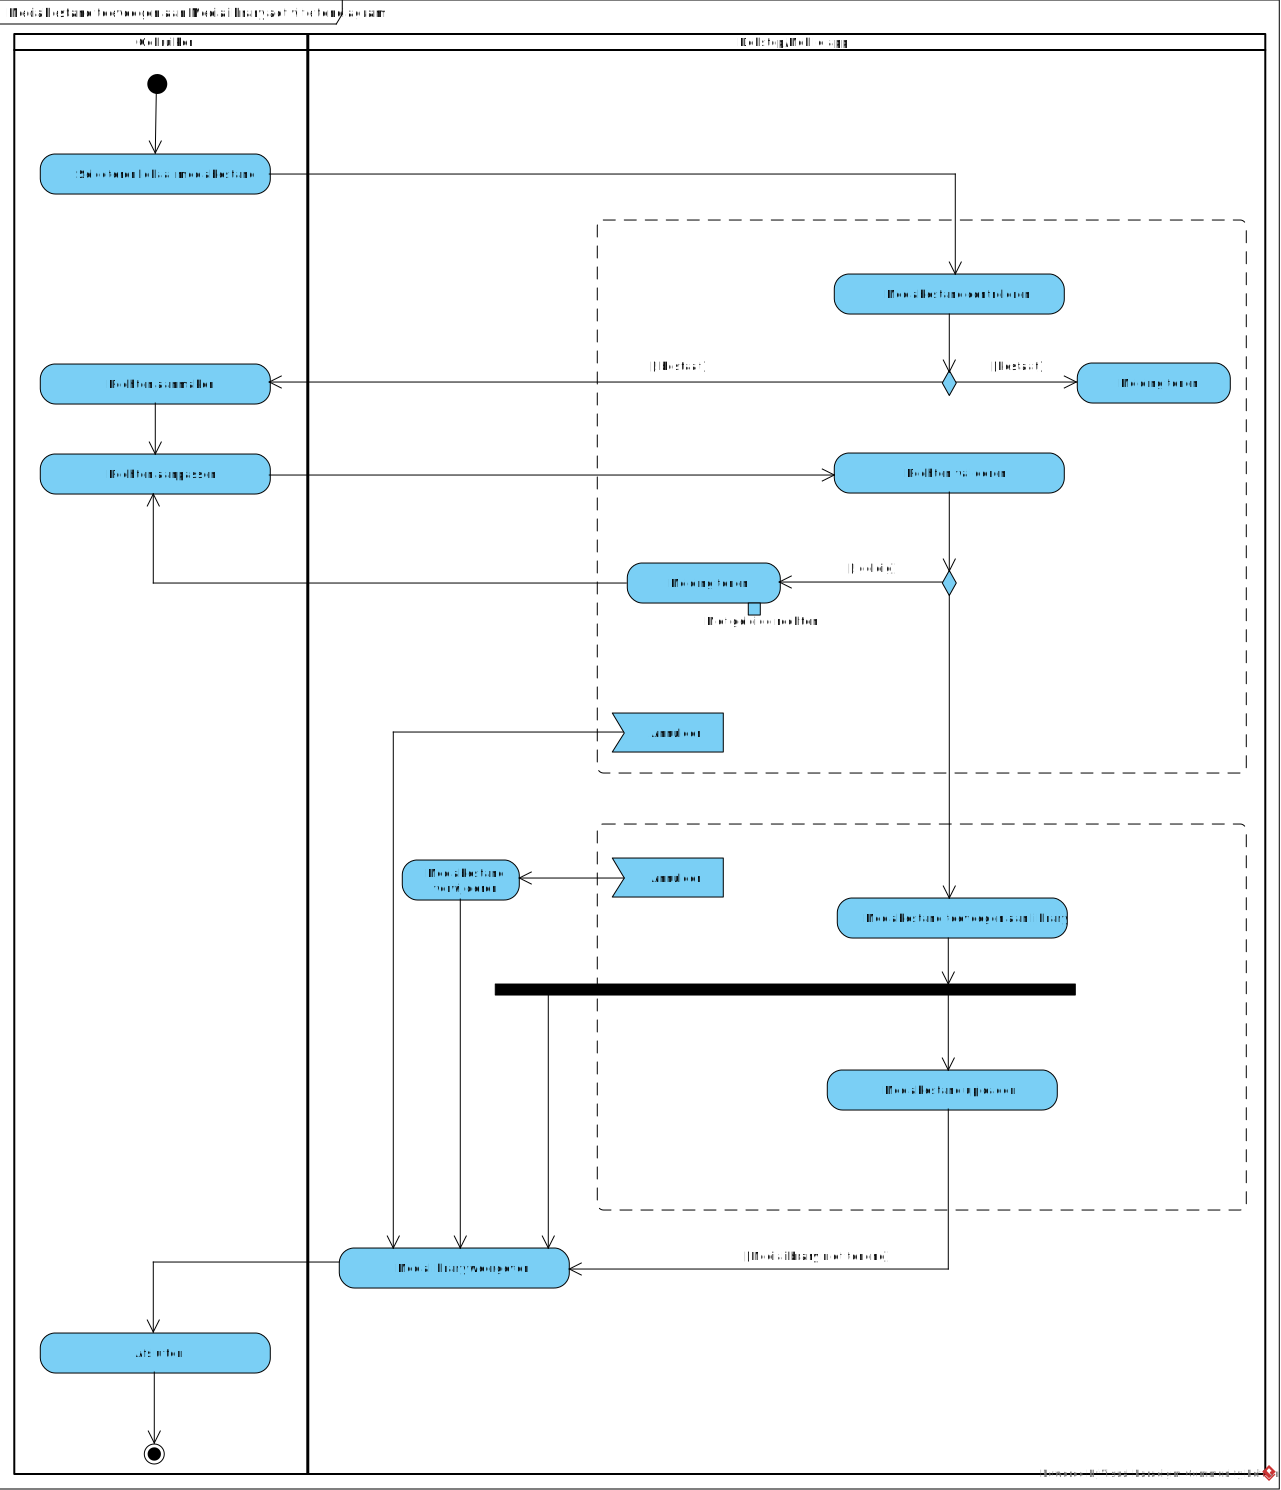
\includegraphics[width=1\textwidth]{images/activiteitendiagram.png}
  \label{figure:activiteitendiagram}
\end{figure}

\newpage

\section{Statemachinediagram}
\label{sec:statemachine}

Het statemachinediagram toont aan in welke staten de Desktop/Mobile app zich 
bevindt bij het openen van een videomediabestand. 
Het bufferen gebeurt in parallel met het afspelen van het bestand of bij pauze.
Het afspelen lukt enkel met de nodige rechten waardoor een bericht zal getoond worden
indien ze niet geldig zijn.

\begin{figure}[H]
  \centering
  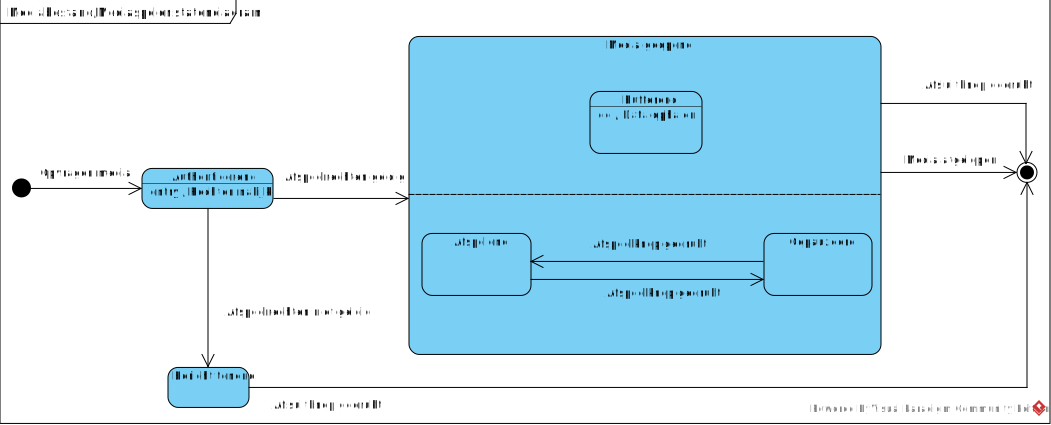
\includegraphics[width=1\textwidth]{images/statendiagram.png}
  \label{figure:statendiagram}
\end{figure}

\newpage

\section{Interactieoverviewdiagram}
\label{sec:interactieoverview}

Het interactie overview diagram beschrijft hoe de admin accounts kan beheren. 
In het begin kan de admin de keuze maken om een nieuw account aan te maken of 
door bestaande accounts te browsen. Bij het browsen kan hij de keuze maken om 
een account te verwijderen of aan te passen. Na een van deze handelingen gaat 
het diagram terug naar de begin interactie waar je terug accounts kan beheren 
of kan kiezen om de interactie te beëindigen (cancel).

\begin{figure}[H]
  \centering
  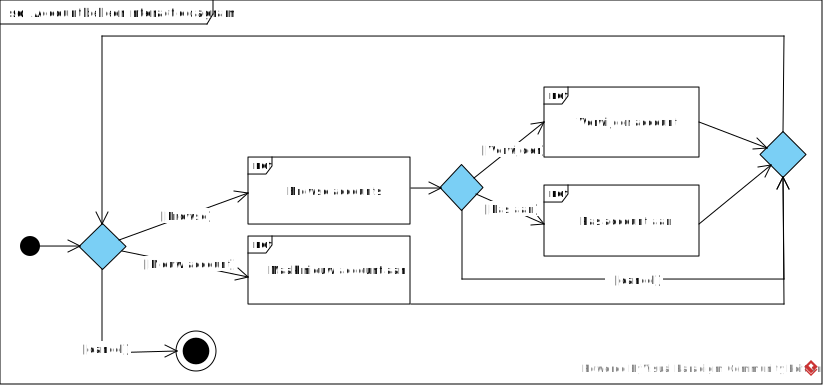
\includegraphics[width=1\textwidth]{images/interactiediagram.png}
  \label{figure:interactiediagram}
\end{figure}
